\chapter{\glsentrytext{DIPolUF} -- three colour \glsentrytext{EM} \glsentrytext{CCD} polarimeter}
\section{Optical design}
\label{sec:dipol-uf}
\begin{figure}
    \centering
    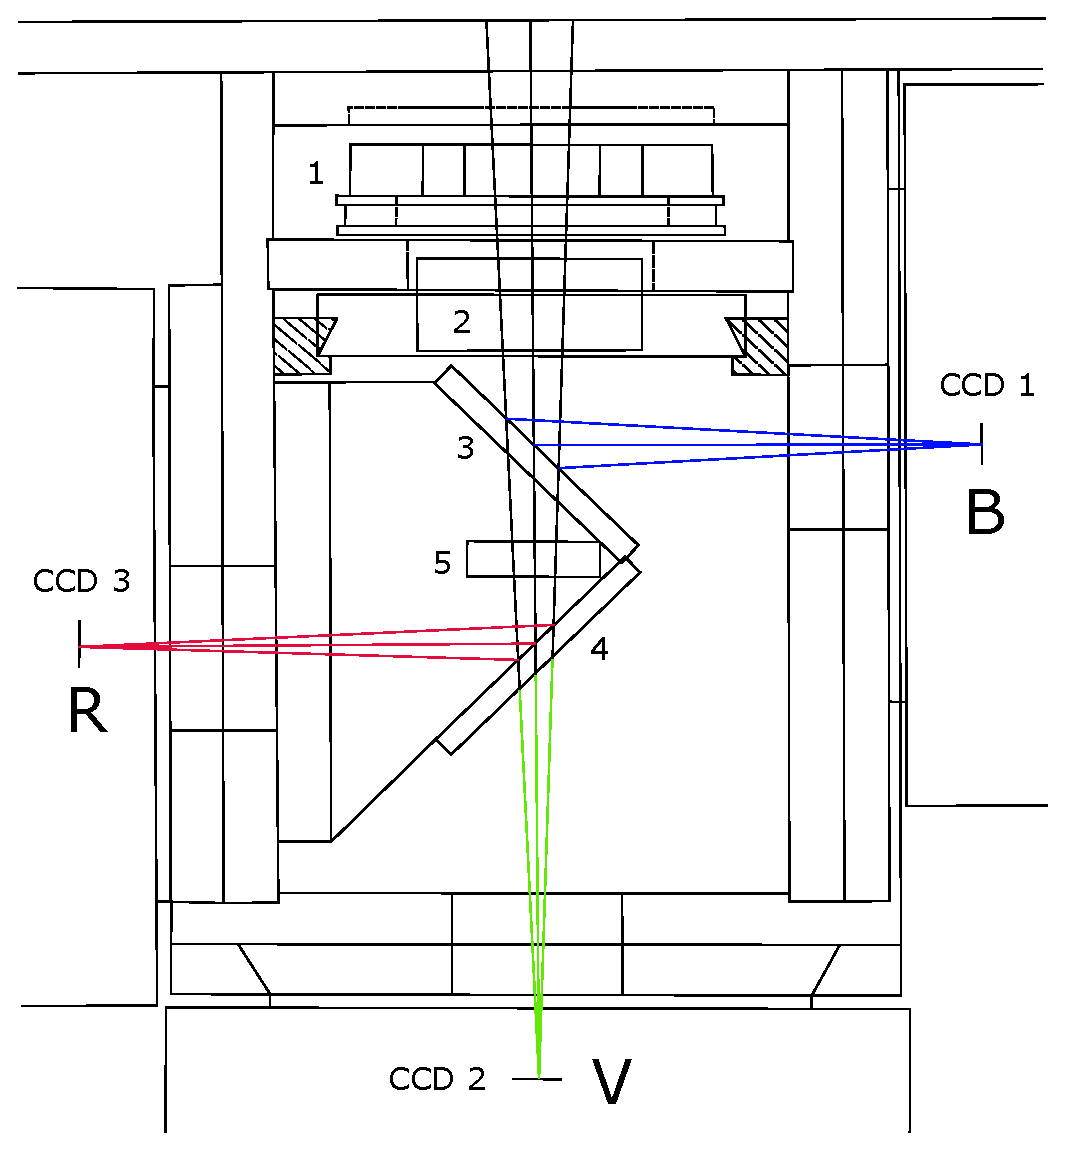
\includegraphics[keepaspectratio, width = 1\linewidth]{images/dipol-uf.eps}
    \caption{ 
        Schematic representation of the side view of \DUF. 
        1. Modulator -- a retarder plate (either $\lambda/2$ or $\lambda/4$), rotated by a stepper motor.
        2. Polarization analyzer - a calcite unit, retractable by another stepper motor.
        3. First dichroic beam-splitter (blue reflector).
        4. Second dichroic beam-splitter (red reflector).
        5. Focal extender lens.}
    \label{fig:dipol-uf-optics}
\end{figure}
The success of the \DP-family polarimeters (see e.g. \citealt{Piirola2020}) led to the development of a new optical polarimeter based on a well-tested design of \DP\ \citep{Piirola2014}.
The new instrument -- named \DUF\ (\textbf{D}ouble \textbf{I}mage \textbf{Pol}arimeter -- \textbf{U}ltra \textbf{F}ast, \paperI) -- makes use of the superachromatic half-wave plate as the modulator and plane-parallel calcite plate as the polarizing beam splitter (analyzer, see Fig.~\ref{fig:dipol-uf-optics}).
Owing to its analyzer, which produces two orthogonally polarized rays of each star in the observed field, the polarimeter records both orthogonally polarization images of the target in three bands simultaneously by means of three top-of-the-line iXon Ultra 897 \gls{EM} \glspl{CCD}, manufactured by ANDOR.
The wavelength separation is achieved with  two dichroic beam-splitters.
The presence of the focal extender lens reduces the field of view in $V$- and $R$-bands, compared to $B$-band.


The polarization modulation is achieved by discrete (i.e., step-by-step) rotation of the modulator (see Sec.~\ref{sec:pol:mods}). 
For linear polarization measurements the rotation step is $22\fdg5$  (using \gls{HWP}), while for circular polarization it is $90^\circ$ \citep[using \gls{QWP}, ][]{Berdyugin2019}.
Following the design of \DP, the orientation of the modulator in \DUF\ is changed by a stepper motor, which is capable of moving the modulator by $22\fdg5$  under $0.250$~s, effectively imposing the upper limit on the time resolution.
\DUF\ features a second stepper motor, which controls position of the analyzer -- it allows to move calcite plate out of the instrument optical axis, turning it into standard imaging optical photometer.


\section{\glsentrytext{EM} \glsentryplural{CCD}}
Each iXon Ultra 897 camera installed in \DUF\ has an active area of $512 \times 512$ pixels ($16 \times 16~\mu\mrm{m}$) used for light exposure and masked storage area of the same size to which the acquired image can be shifted immediately after the end of exposure.
Thus, when used in `Frame Transfer' mode, the time between two subsequent exposures is greatly reduced by staring the next exposure at the same time when the already acquired image is transferred from the masked area to the read out register.
\DUF\ makes use of two output amplifiers available in each camera: conventional and electron-multiplication.
The conventional amplifier, which provides the best dynamic range (limited by the analog-to-digital converter), is best suited for observing bright targets.
Using the defocusing technique it is possible to collect up to $10^8$ \glspl{ADU} for a sufficiently bright target without saturation, pushing the limiting accuracy of \DUF\ toward $10^{-6}$, an order of magnitude better than that of its predecessor, \DP\ \paperIp.
The variable gain \gls{EM} amplifier is perfect for faint targets, where single-photon sensitivity can play an important role.


iXon Ultra 897 are highly configurable cameras and each parameter can be adjusted in real time using software tools provided by the manufacturer.
Exposure time, readout rates (horizontal shift speed and vertical shift rate), readout regime (full image, sub- or binned image), trigger mode (software or external hardware), acquisition mode (single scan, accelerated kinetic / fast kinetic series, hardware-supported accumulation series, or their combinations), amplifiers and their gains can be modified to meet the requirements of a particular scientific task.
Optimal combinations of settings, such as e.g. fast readout speeds, allow cameras to take up to 56 full frame (no binning) images per second, if operated in `Frame Transfer' regime, which is more than enough to match the modulator rotation rate, or provide good time resolution in photometric regime. \DUF\ is designed to operate within three optical ($BVR$) filters, at $\lambda = 450, 545, 650$~nm; it uses `BV' coating modification of the 897 series cameras that are more sensitive in the blue wavelength range for the $B$-band, compared to `EX' coating used for the $V$ and $R$ bands and optimized for \gls{ONIR} wavelength range.




\section{Control hardware and software}
\begin{figure}
    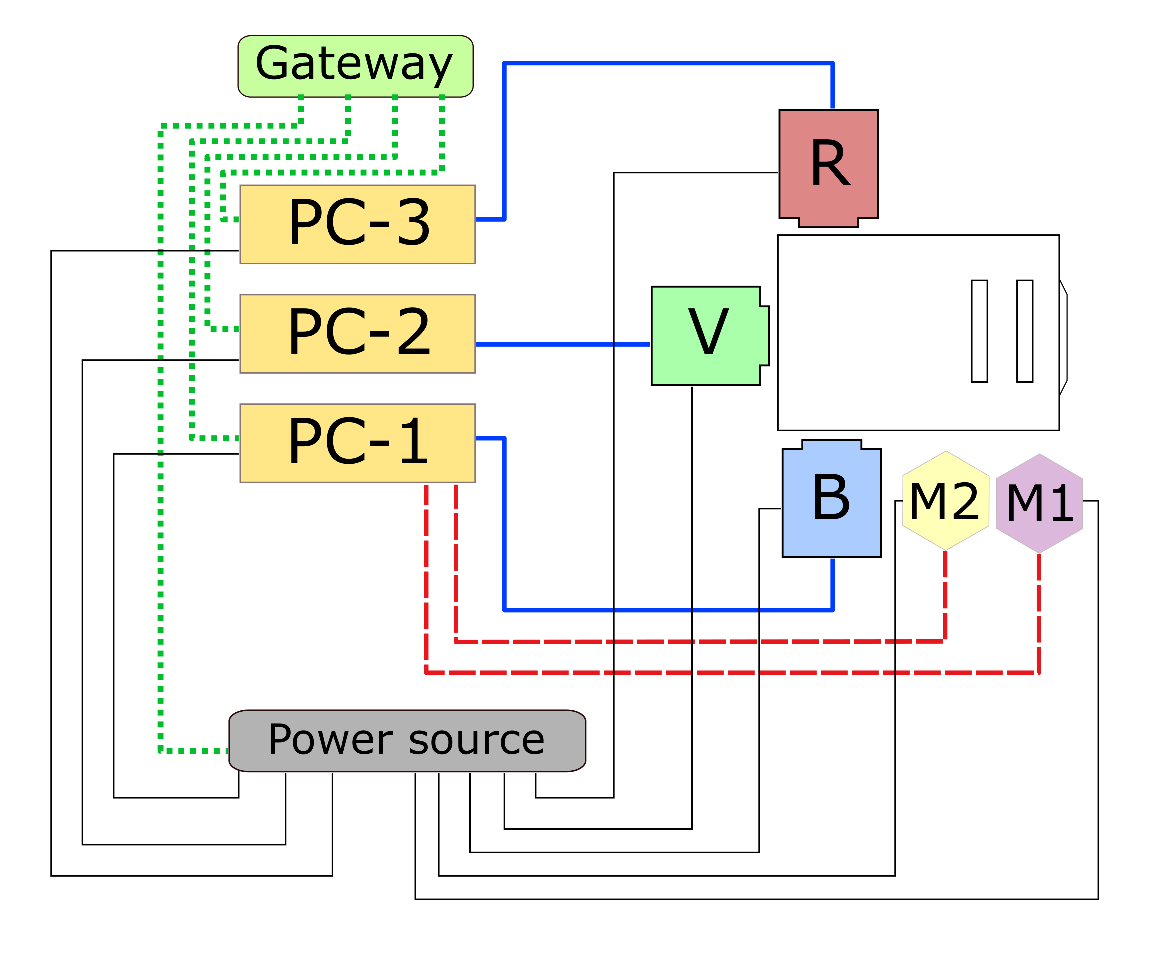
\includegraphics[keepaspectratio, width = 0.49\linewidth]{images/hardware.eps}
    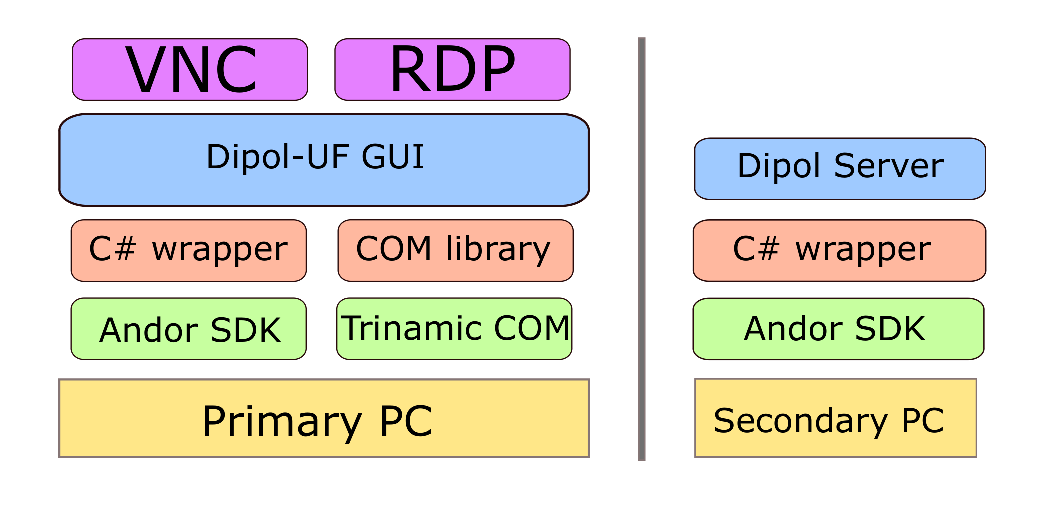
\includegraphics[keepaspectratio, width = 0.49\linewidth]{images/software.eps}
    \caption{
        Left panel: schematic representation of \DUF\ control hardware and their interconnections.
        Right panel: schematic representation of the software that operates \DUF.
        See \paperI.}
    \label{fig:dipol-uf-components}

\end{figure}
\DUF\ is a much more complicated instrument compared to \DP, mainly due to the new \gls{EM} \glspl{CCD} used to build it.
A detailed overview of \DUF\ is given in \paperI.
As a result, the simple setup of one control computer connected to three cameras of \DP, running all control software simultaneously, was no longer an option.
Each camera of \DUF\ is controlled by a dedicated industrial-grade control computer, which are united into a local area network operated by a special router.
Two \glspl{PC} act as secondary machines (see `\gls{PC}-2' and `\gls{PC}-3' in Fig.~\ref{fig:dipol-uf-components}) and provide remote access to their respective cameras to the main computer (`\gls{PC}-1') within the local network.
Main computer runs the custom control software, created specifically for \DUF, which is responsible for providing \gls{GUI} for the observers, managing camera configurations, operating the modulator and analyzer stepper motors, synchronously controlling image acquisition process in all three cameras, and storing data retrieved from the cameras in a format suitable for astronomical data reduction pipelines, such as \gls{FITS}.

Inspired by the successful remote operations of \DP, \DUF\ was designed to be a fully remotely controlled instrument.
Each hardware component is powered through a remotely controlled \gls{PDU}, and therefore can be switched on/off independently of other components of the instrument.
To facilitate safe remote access, \DUF\ computers are put behind a router, which acts as a gateway, isolating the instrument from potential threats.
The router provides an authorization mechanism for remote observers using industry-standard \gls{VPN} protocols.
As a result, full cycle of \DUF\ polarimetric observations can be carried out in a fully remote regime, including instrument start up and shut down, image acquisition and data transfer, which proved to be exceptionally useful when observers' travelling capabilities are limited.


Although there are several solutions available on the market that provide means for combining multiple cameras connected to multiple computers into one instrument, none of these third-party products were found to be suitable for \DUF\ operations.
As a result, \DUF\ has its own control software that takes care of all \DUF\ processes.
The control software (and its components) are build using \texttt{C\#} programming language targeting Microsoft's .NET Framework 4.8, a framework that provides managed runtime and a set of libraries for memory-safe development under Windows.
Two secondary computers run special servers that expose \gls{RPC} \glspl{API}, available via \gls{TCP} (see Fig.~\ref{fig:dipol-uf-components}, right panel).
The network intercommunication is built on \gls{WCF}.
The main computer runs a different application that acts as a client, connecting to other machines within local network.
It also issues commands to the stepper motors (`M1' and `M2' in Fig.~\ref{fig:dipol-uf-components}) via standard serial interfaces.
The \gls{GUI} is build within the same framework, using \gls{WPF}.
With the help of third-party remote desktop and collaboration tools, such as \gls{VNC}, \DUF's \gls{GUI} can be accessed by several observers simultaneously regardless of their geographical position, which allows demonstration of \DUF\ operations to students or colleagues from foreign institutions, interested in the instrument.

\section{Data reduction and polarization measurement}
\label{sec:data_red}
\begin{figure}
    \centering
    \includegraphics[keepaspectratio, width = 0.9\linewidth]{images/MAXI_Conv_Pol.png}
    \caption{
        Field around \MAXI\ \citep{Kawamuro2018, Denisenko2018} as seen through \DUF\ control software, July 2019.
        With analyzer in place, each star in the field produces two images, ordinary and extraordinary, which for \MAXI\ are marked with `o' and `e', respectively.
        }
    \label{fig:dipol-uf-maxi}
\end{figure}
Images, obtained by a dual-image polarimeter (such as \DP\ or \DUF), typically resemble that shown in Fig.~\ref{fig:dipol-uf-maxi}.
It is possible to model the propagation of light through the instrument and establish relationship between the brightness of ordinary and extraordinary rays recorded by the polarimeter and polarization of the incident light.
This relationship can be expressed in terms of Mueller calculus:
\begin{equation}
    \vctr{S}_\mrm{det} = \vctr{S}_0 + \mtrx{M}_\mrm{inst} \left(\vctr{S}_\mrm{dome} + \mtrx{M}_\mrm{tel} \left(\vctr{S}_\mrm{back} + \vctr{S}_\mrm{inc}\right)\right),
\end{equation}
where $\vctr{S}_\mrm{det}$ is the vector of Stokes parameters of the light at the detector, $\vctr{S}_0$ represents zero-point calibration error of the detector,  $\mtrx{M}_\mrm{inst}$ describes how light is transformed by the polarimeter, $\vctr{S}_\mrm{dome}$ and $\mtrx{M}_\mrm{tel}$ describe contribution of the dome and telescope, $\vctr{S}_\mrm{back}$ stands for background polarization (e.g., from the sky), and $\vctr{S}_\mrm{inc}$ is the vector of Stokes parameters of the incident light, the quantity that needs to be measured \citep{AstronomicalPolarimetry}.
As was discussed before, detectors are usually capable of recording the intensity of the incoming radiation, and not its Stokes parameters, thus leaving observers with only one Stokes parameter -- $I_\mrm{det}$.

Let us consider a simplified formula, assuming that neither dome nor telescope affect significantly the Stokes parameters of the incident light:
\begin{equation}
    \label{eq:dipol-uf:data_proc:gen_form}
    \vctr{S}_\mrm{det}^\prime =  \mtrx{M}_\mrm{inst} \vctr{S}_\mrm{inc}^\prime.
\end{equation}
The instrument, in turn, consists of two primary optical components -- the modulator and the analyzer.
The (ideal) modulator is represented with a matrix operator $\mtrx{M}_\mrm{mod}(\phi)$, where $\phi$ is the introduced phase delay between orthogonally polarized components (such that for half-wave plate $\phi = \pi$, see \citealt{PolarizedLight2}):

\begin{equation}
    \mtrx{M}_\mrm{mod}(\phi) =
    \begin{bmatrix}
    1 & 0 & 0 & 0 \\
    0 & 1 & 0 & 0 \\
    0 & 0 & \cos\phi & \sin\phi \\
    0 & 0 & -\sin\phi & \cos\phi \\    
    \end{bmatrix}.
\end{equation}
The discrete rotation of the modulator by an arbitrary angle $\varphi$ is expressed as $\mtrx{M}_\mrm{rot}(-\varphi) \cdot \mtrx{M}_\mrm{mod}(\phi) \cdot \mtrx{M}_\mrm{rot}(\varphi)$ \citep{PolarizedLight2}, and
\begin{equation}
    \mtrx{M}_\mrm{rot}(\varphi) =
    \begin{bmatrix}
    1 & 0 & 0 & 0 \\
    0 & \cos2\varphi & \sin2\varphi & 0 \\
    0 & -\sin2\varphi & \cos2\varphi & 0 \\
    0 & 0 & 0 & 1
    \end{bmatrix}.
\end{equation}

In order to describe the dual-beam analyzer (a plane parallel calcite plate as used in \DUF), two operators are required -- one per each orthogonally polarized beam propagating through the optical component.
The general form of such operator, $\mtrx{M}_\mrm{pol}(a, \gamma)$, is
\begin{equation}
    \mtrx{M}_\mrm{pol}(a, \gamma) = 
    \frac{a^2}{2}
    \begin{bmatrix}
        1 & \cos2\gamma & 0 & 0 \\
        \cos2\gamma & 1 & 0 & 0 \\
        0 & 0 & \sin2\gamma & 0 \\
        0 & 0 & 0 & \sin2\gamma \\
    \end{bmatrix},
\end{equation}
where $\gamma$ describes the polarization angle, such that emission, polarized in this direction, is allowed through, and $a \le 1$ is the transmission coefficient \citep{Piirola_Thesis, PolarizedLight2}.
Thus, the transmission of ordinary ray can be approximated with $\mtrx{M}_\mrm{pol}(a, 0)$, while extraordinary ray propagates in accordance with $\kappa \mtrx{M}_\mrm{pol}(a, \pi/2)$.
Here $\kappa$ represents the ratio between the intensities of the ordinary and extraordinary rays, which is exactly unity in the ideal case, but departs from this value in real optical systems.

Finally, Eq.~\ref{eq:dipol-uf:data_proc:gen_form} can be expressed (following the rules of non-commutative matrix multiplication) in the following form:
\begin{equation}
    \label{eq:dipol-uf:final_relation}
    \vctr{S}_\mrm{det}^\prime =  \left[\mtrx{M}_\mrm{pol}(a, \gamma_\mrm{o,e})\cdot \mtrx{M}_\mrm{rot}(-\varphi) \cdot \mtrx{M}_\mrm{mod}(\phi) \cdot \mtrx{M}_\mrm{rot}(\varphi)\right] \vctr{S}_\mrm{inc}^\prime.
\end{equation}


Intensities of the recorded stellar images can then be extracted with the help of aperture photometry.
With Eq.~\ref{eq:dipol-uf:data_proc:gen_form} derived, it is now possible to express the intensity of the ordinary and extraordinary rays on the detector in terms of the incident Stokes parameters.
Bearing in mind that \DUF\ uses half-wave plate as modulator when measuring linear polarization (the default scenario), $ \mtrx{M}_\mrm{inst}$ for the ordinary and extraordinary rays is simply:
\begin{equation}
    \begin{matrix}
        \mtrx{M}_\mrm{inst}^\mrm{o}(a, \varphi) = & \mtrx{M}_\mrm{pol}(a, 0)\cdot \mtrx{M}_\mrm{rot}(-\varphi) \cdot \mtrx{M}_\mrm{mod}(\pi / 2) \cdot \mtrx{M}_\mrm{rot}(\varphi), \\
        \mtrx{M}_\mrm{inst}^\mrm{e}(a, \varphi) = & \mtrx{M}_\mrm{pol}(a, \pi / 2)\cdot \mtrx{M}_\mrm{rot}(-\varphi) \cdot \mtrx{M}_\mrm{mod}(\pi / 2) \cdot \mtrx{M}_\mrm{rot}(\varphi).
    \end{matrix}
\end{equation}
Assuming the incident Stokes parameters are denoted as $[I, Q, U, V]^\mrm{T}$ and that
\begin{equation}
    {\vctr{S}_\mrm{det}^\mrm{o,e}}^\prime = \mtrx{M}_\mrm{inst}^\mrm{o, e}(a, \varphi) \cdot [I, Q, U, V]^\mrm{T},
\end{equation}
the following relationship is obtained:
\begin{eqnarray}
    \label{eq:dipol-uf:data_proc:stokes_detector_o}
    {\vctr{S}_\mrm{det}^\mrm{o}}^\prime  = & 
    \frac{a^2}{2}
    \begin{bmatrix}
        I + Q\cos4\varphi + U\sin4\varphi\\
        I + Q\cos4\varphi + U\sin4\varphi \\
        0 \\ 
        0 \\
    \end{bmatrix}, \\
    \label{eq:dipol-uf:data_proc:stokes_detector_e}
    {\vctr{S}_\mrm{det}^\mrm{e}}^\prime  = & 
    \kappa \frac{a^2}{2}
    \begin{bmatrix}
        I - Q\cos4\varphi - U\sin4\varphi\\
        - I + Q\cos4\varphi + U\sin4\varphi \\
        0 \\ 
        0 \\
    \end{bmatrix}.
\end{eqnarray}
It is immediately evident that both rays are fully linearly polarized, but in orthogonal direction.
The total intensity of the two light beams reaching detector is 
\begin{equation}
    \frac{a^2}{2} \left( I(1 + \kappa) + (Q\cos4\varphi + U\sin4\varphi)(1 - \kappa)\right),
\end{equation}
which is equal to incident $I$ if the analyzer splits incoming light equally ($\kappa = 1$) and the transmission coefficient $a$ is unity.


If the incident radiation is (partially) linearly polarized to a degree $p$ at a polarization angle $\theta$, then intensities, extracted from Eqs.~\ref{eq:dipol-uf:data_proc:stokes_detector_o},\ref{eq:dipol-uf:data_proc:stokes_detector_e} are
\begin{equation}
    \begin{aligned}
        \begin{aligned}
            I_\mrm{det}^\mrm{o}(\varphi) =& \frac{a^2}{2}\left(I + Q\cos4\varphi + U\sin4\varphi\right) = \\
            &\frac{a^2}{2} I \left(1 + p\cos\left(4\varphi - 2\theta\right)\right),
        \end{aligned}\\
        \begin{aligned}
            I_\mrm{det}^\mrm{e}(\varphi) =& \kappa\frac{a^2}{2}\left(I - Q\cos4\varphi - U\sin4\varphi\right) = \\
            &\kappa\frac{a^2}{2} I \left(1 - p\cos\left(4\varphi - 2\theta\right)\right). 
        \end{aligned}
    \end{aligned}
\end{equation}

To avoid photometric calibrations necessary for obtaining absolute fluxes, a ratio of extraordinary and ordinary intensities can be considered.
This ratio, $R(\varphi) = I_\mrm{det}^\mrm{e}(\varphi)/I_\mrm{det}^\mrm{o}(\varphi)$ \citep{Clarke1971}, is insensitive to changes in the atmospheric seeing and other similar effects, as both rays are measured simultaneously under the exactly same conditions.
Even though the absolute detected intensity may vary from image to image, the ratio remains stable and reflects the polarimetric properties of the source.


$R(\varphi)$ contains an unknown factor, $\kappa$, which remains constant throughout the observational cycle, but otherwise is unknown prior to the data processing phase.
It can be shown that for relatively small (such as observed in astrophysical objects) polarization, $\kappa = \frac{1}{4n}\sum_{j = 0} ^ {4n - 1} R(j \pi/8 )$ is the average value of $R$ \citep[see, e.g.,][]{Piirola_Thesis}.
Using series expansion, applied to $\kappa \frac{1 + p\cos\left(4\varphi - 2\theta\right)}{1 - p\cos\left(4\varphi - 2\theta\right)}$, and denoting $R(j \pi /8) \equiv R_j$, the observed normalized Stokes parameters are \citep{Piirola_Thesis}:
\begin{equation}
    \begin{aligned}
        q &= p\cos2\theta = \frac{1}{4n\kappa}\sum_{j = 0}^{n - 1} \left(R_{4j} - R_{4j + 2}\right),\\
        u &= p\sin2\theta = \frac{1}{4n\kappa}\sum_{j = 0}^{n - 1} \left(R_{4j + 1} - R_{4j + 3}\right), \\
        \kappa &= \frac{1}{4n}\sum_{j = 0}^{n - 1} \left(R_{4j} + R_{4j + 1} + R_{4j + 2} + R_{4j + 3}\right).
    \end{aligned}
\end{equation}

Thus, the formulae used with \DP\ and \DUF\ are derived if $n$ is chosen to be equal to unity \citep[see][]{Berdyugin2019}.
A single measurement of the observed Stokes $q$ and $u$ parameters is obtained using a minimum of four sequential polarimetric images, resulting into four independent polarimetric measurements of both parameters per one full rotation of the modulator (which performs it in 16 steps).
Examples of other data reduction procedures and their comparisons can be found in e.g. \citet{Bagnulo2009}.

\begin{figure}
    \centering
    \includegraphics[keepaspectratio, width = 1\linewidth]{images/duf_weights.pdf}
    \caption{The distribution of the weights applied to the individual Stokes parameters during the averaging procedure.}
    \label{fig:dipol-uf:weights_dist}
\end{figure}

After $q_i$ and $u_i$ individual measurements are collected ($i$ being the index of the measurement, running from $1$ to $N$), a special weighting algorithm is applied, which is designed to be insensitive to the outliers by assigning smaller weights to such values.

The procedure is iterative, at each step $j$ the following quantities are defined:
\begin{itemize}
    \item $ \langle q_j \rangle  = \sum_{i = 1}^N w_q^{i,j} q_i$ is the average $q$ parameter,
    \item $ \langle u_j \rangle  = \sum_{i = 1}^N w_u^{i,j} u_i$ is the average $u$ parameter,
    \item $w_q^{i,j}$ are weights used to calculate $ \langle q_j \rangle $, and $\Sigma_q^j = \sum_i w_q^{i,j}$ is their sum,
    \item $w_u^{i,j}$ and $\Sigma_u^j = \sum_i w_u^{i,j}$ are similar quantities used to obtain $ \langle u_j \rangle $,
    \item $\sigma_q^j = \left(\sum_{i = 1}^N w_q^{i,j} \left(q_i -  \langle q_j \rangle \right)^2 / \Sigma_q^j \right)^{1/2}$ is the independent weighted standard deviation of $q_i$,
    \item $\sigma_u^j = \left(\sum_{i = 1}^N w_u^{i,j} \left(u_i -  \langle u_j \rangle \right)^2 / \Sigma_u^j \right)^{1/2}$ is its counterpart for $u_i$,
    \item $ \langle \sigma_j \rangle  = \sqrt{\left(\left(\sigma_q^j\right)^2 + \left(\sigma_u^j\right)^2\right)/ \left(\Sigma_q^j + \Sigma_u^j - 2\right)}$ gives an estimate of the standard error of the mean $p_j$ when $q_i$ and $u_i$ are obtained from the same set of measurements \citep{Serkowski1962},
    \item $\sigma_j =  \langle \sigma_j \rangle \sqrt{\frac{1}{2}\left(\Sigma_q^j + \Sigma_u^j\right)}$ is an estimate of the weighted standard deviation.
\end{itemize}
The weights depend on the distances $d_q^{i, j} = \left|q_i -  \langle q^j \rangle \right|$ and $d_u^{i, j} = \left|u_i -  \langle u_j \rangle \right|$ in the following way:
\begin{equation}
    w_q^{i,j} = 
    \begin{cases}
        1,&~d_q^{i, j} \le 2 \sigma_j, \\
        \frac{1}{\left(2 d_q^{i, j} / \sigma_j - 3\right)^2},&~ 2\sigma_j < d_q^{i, j} < 3\sigma_j, \\
        0,&~d_q^{i,j} \ge 3\sigma_j.
    \end{cases}
\end{equation}
$w_u^{i, j}$ are obtained similarly.
Fig.~\ref{fig:dipol-uf:weights_dist} shows how applied weight changes with the distance $d$, expressed in units of standard deviation $\sigma$.

The iterative process continues until $ \langle q_j \rangle $ and $ \langle u_j \rangle $ reach their optimal values, i.e. these average quantities do not change when transitioning to the next step (e.g., $\left| \langle q_j \rangle  -  \langle q_{j + 1} \rangle  \right| \ll \epsilon$, where $\epsilon$ is a threshold).
At this point, $ \langle q_j \rangle $, $ \langle u_j \rangle $, and $ \langle \sigma_j \rangle $ are taken to be the mean reduced Stokes parameters $ \langle q \rangle $, $ \langle u \rangle $ and their standard error $ \langle \sigma \rangle $, from which both polarization angle and polarization degree can be obtained using, e.g., classical estimators \citep{Serkowski1962, NaghizadehKhouei1993}:

\begin{equation}
    \begin{aligned}
         \langle p \rangle  =& \sqrt{ \langle q \rangle ^2 +  \langle u \rangle ^2}, \\
         \langle \theta \rangle  =& \frac{1}{2}\arctan \frac{ \langle u \rangle }{ \langle q \rangle }, \\
        \sigma_{ \langle p \rangle } =& 
            \begin{cases}
                 \langle \sigma \rangle \left(2 - \frac{\pi}{2}\right)^{1/2} &\mathrm{when}~p \approx 0, \\
                 \langle \sigma \rangle  &\mathrm{when}~p \gg  \langle \sigma \rangle ,
            \end{cases} \\
        \sigma_{ \langle \theta \rangle } =& 
            \begin{cases}
                \frac{\pi}{\sqrt{12}} &\mathrm{when}~p \approx 0, \\
                \frac{1}{2}\frac{ \langle \sigma \rangle }{ \langle p \rangle } &\mathrm{when}~p \gg  \langle \sigma \rangle ,
            \end{cases}
    \end{aligned}
\end{equation}
where $p$ is the true polarization degree unknown to the observer.
For sufficiently large \gls{SNR}, $p /  \langle \sigma \rangle $, it is safe to assume $ \langle p \rangle  \equiv p$ and $ \langle \theta \rangle  \equiv \theta$.
For $\mathrm{SNR} \le 3$ \citep[based on numerical simulations, see, e.g.,][]{Montier2015} the difference between $ \langle p \rangle $ and $p$ becomes substantial.
In the limiting case of $p \equiv 0$ ($ \langle q \rangle  = 0,~ \langle u \rangle  = 0$), computed value of $ \langle p \rangle  \neq 0$, leading to the overestimation of the observed polarization.
This problem is partially solved by polarization estimators $\hat{p}\left( \langle p \rangle , \sigma_{ \langle p \rangle }\right)$ \citep{Simmons1985}, which are designed to provide better measurements of $p$ compared to $ \langle p \rangle $, especially when \gls{SNR} is low.
A detailed comparison of widely-used polarization degree estimators is given in \citet{Montier2015a}.

At low \gls{SNR}, the distribution of $p$ becomes highly asymmetric and deviates from the normal distribution, which has profound implications for the \gls{CI} calculations.
For any \gls{SNR} the \glspl{CI} can be obtained using the integration method of \citet{Simmons1985}, applied either separately to polarization degree \citep{Vaillancourt2006} and polarization angle \citep{NaghizadehKhouei1993}, or to the joint 2D distribution of $\hat{p}$ and $\hat{\theta}$ \citep{Montier2015}.
From \gls{SNR} $\approx 6$ and onward, it is safe to assume $\hat{p}\sim \mathcal{N}( \langle p \rangle  ^ *,  \langle \sigma \rangle )$ and $\hat{\theta}\sim \mathcal{N}( \langle \theta \rangle , \sigma_{ \langle \theta \rangle })$, where $ \langle p \rangle  ^ * \le  \langle p \rangle  $ is the de-biased estimate of true polarization, such that $ \langle p \rangle  ^ * \to  \langle p \rangle $ when $\mathrm{SNR} \to \infty$.
Owing to the sensitivity of \DUF, the typical value of \gls{SNR} is about 10 for faint targets, such as \glspl{LMXB}. 
As a result, the \glspl{CI} are symmetric and can be easily constructed as $[ \langle p \rangle  - \kappa \sigma_{ \langle p \rangle };~ \langle p \rangle  + \kappa \sigma_{ \langle p \rangle }]$ and $[ \langle \theta \rangle  - \kappa \sigma_{ \langle \theta \rangle };~ \langle \theta \rangle  + \kappa \sigma_{ \langle \theta \rangle }]$, where $\kappa$ determines the width of the interval.
The standard 1$\sigma$ intervals are obtained when $\kappa = 1$.

The final step in the data reduction procedure is calibration.
The contribution of the optical components of the telescope and polarimeter to the observed polarization is collectively described by $\mtrx{M}_\mrm{inst}$ in Eq.~\ref{eq:dipol-uf:data_proc:gen_form}.
In case of linear polarization, this can lead to changes in the zero-point polarization angle, polarization scale, as well as to systematic errors in $q$ and $u$ reduced Stokes parameters \citep{Berdyugin2019}.
The polarization, introduced by the polarimeter itself, can be eliminated by rotating the instrument as a whole through 360$^\circ$, measuring polarization of the source at different instrument orientations.
Alternatively, a rotating retarder can be used.
Averaging measurements over one full rotation cancels out the majority of the internal polarimeter polarization which manifest itself as spurious sinusoidal modulations.
The polarization scale coefficient can be determined using a dedicated scale calibration component installed in front of the instrument, which is important especially in the case of inefficient modulators.

Instrument polarization produced by the telescopes cannot be easily eliminated.
However, telescopes with alt-azimuthal mounting have a constantly rotating field and, as a result, rotating polarized image of the sky.
The modulations, introduced by the telescope motion, can be modelled and subtracted from the observed $q$ and $u$ parameters.
Equatorial telescopes contribute constant offsets to $q$ and $u$, which are independent of the equatorial coordinates of the observed target.
This bias cannot be eliminated without proper observations of the sources which have no linear polarization.

If the instrument polarization $[q_i, u_i]^\mrm{T}$ is sufficiently small, the relationship between the incident $[q_0, u_0]^\mrm{T}$ and detected $[q, u]^\mrm{T}$  linear polarization is expressed as follows:
\begin{equation}
    \label{eq:pol_calib}
    \begin{bmatrix}
        q\\u
    \end{bmatrix} = f
    \begin{bmatrix}
        \cos 2\varphi & -\sin 2\varphi \\
        \sin 2\varphi & \cos 2\varphi
    \end{bmatrix}
    \begin{bmatrix}
        q_0\\ u_0
    \end{bmatrix} +
    \begin{bmatrix}
        q_i \\ u_i
    \end{bmatrix},
\end{equation}
where $f$ is the scaling factor, $\varphi$ is the offset of the polarization angle zero-point.
These calibration parameters can be determined by observing standard stars.
A large sample of zero-polarized stars ($q_0 \approx u_0 \approx 0$) give an estimate of the average systematic telescope polarization $[q_i, u_i]^\mrm{T}$ \citep{Piirola2020}.
With instrument polarization known, the scaling factor and zero-point of polarization angle are inferred from observations of high-polarization standards with known polarization degree and angle.
To account for possible variability of standard stars, Eq.~\ref{eq:pol_calib} is solved simultaneously for several stars, yielding the best-fit values of $f$ and $\varphi$.

The instrument polarization can be subtracted either from the individually measured $q_i$ and $u_i$ values, or from the average $ \langle q \rangle $ and $ \langle u \rangle $.
Both Stokes parameters and their errors should be scaled using $f$ after the instrument polarization has been subtracted (the error on the polarization angle is insensitive to polarization scaling).
Finally, the angle calibration is applied by subtracting the zero-point $\varphi$ from the inferred polarization angle, which affects neither polarization degree nor errors.
